\section{コースB: 第IVポジション}
\begin{center}
\begin{tabular}{|lcl|}
\hline
この章の基礎練習 & : & 1. 開放弦の練習 2. 「\ref{half_scale}」「\ref{1st_scale}」「\ref{2nd_scale}」の音階練習 3. 「弦楽セレナーデ」\\
この章の修了課題 & : & 1. 「\ref{4th_scale}」の音階練習を正しい音程で暗譜して演奏できる\\ 
               &   & 2. 「マイスタージンガー」を正しい音程で暗譜して演奏できる\\\hline
\end{tabular}
\end{center}

\subsection{第IVポジションの位置}
\begin{flushleft}
\begin{minipage}{280pt}
\ \ \ 親指をネックの一番下まで降ろしてください。その親指の正面を2の指
で押さえます。これが4thポジションです。1と4は2に合わせます。指の間隔は
ハーフポジションと比べてだいぶ狭くなります。このポジションのD、A、E線
で取れる音は、細い方の隣の弦の1stポジションであることを覚えてください。
\subsection{第IVポジションで取れる音}
\begin{music}
\nostartrule
\parindent 0pt
\setclef1{\bass}  
\startpiece
\notes\enotes
\Notes\zchar{18}{G線}\zchar{13}{\bf 1}\wh{d}\zchar{14}{\bf 2}\wh{^d}\zchar{14}{\bf 4}\wh{e}\enotes
\doublebar
\Notes\zchar{13}{\bf 1}\wh{d}\zchar{14}{\bf 2}\wh{_e}\zchar{14}{\bf 4}\wh{=e}\enotes
\doublebar
\Notes\zchar{18}{D線}\zchar{11}{\bf 1}\wh{a}\zchar{11}{\bf 2}\wh{^a}\zchar{11}{\bf 4}\wh{b}\enotes
\doublebar
\Notes\zchar{11}{\bf 1}\wh{a}\zchar{11}{\bf 2}\wh{_b}\zchar{11}{\bf 4}\wh{=b}\enotes
\setdoublebar
\endpiece
\startpiece
\notes\enotes
\Notes\zchar{14}{A線}\zchar{9}{\bf 1}\wh{'E}\zchar{9}{\bf 2}\wh{F}\zchar{9}{\bf 4}\wh{^F}\enotes
\doublebar
\Notes\zchar{9}{\bf 1}\wh{'E}\zchar{9}{\bf 2}\wh{F}\zchar{9}{\bf 4}\wh{_G}\enotes
\doublebar
\Notes\zchar{14}{E線}\zchar{9}{\bf 1}\wh{'B}\zchar{9}{\bf 2}\wh{C}\zchar{9}{\bf 4}\wh{^C}\enotes
\doublebar
\Notes\zchar{9}{\bf 1}\wh{'B}\zchar{9}{\bf 2}\wh{C}\zchar{9}{\bf 4}\wh{_D}\enotes
\setdoublebar
\endpiece
\end{music}
\end{minipage}
\hfill
\begin{minipage}{65pt}
\addtocounter{figure}{1}
\begin{center}
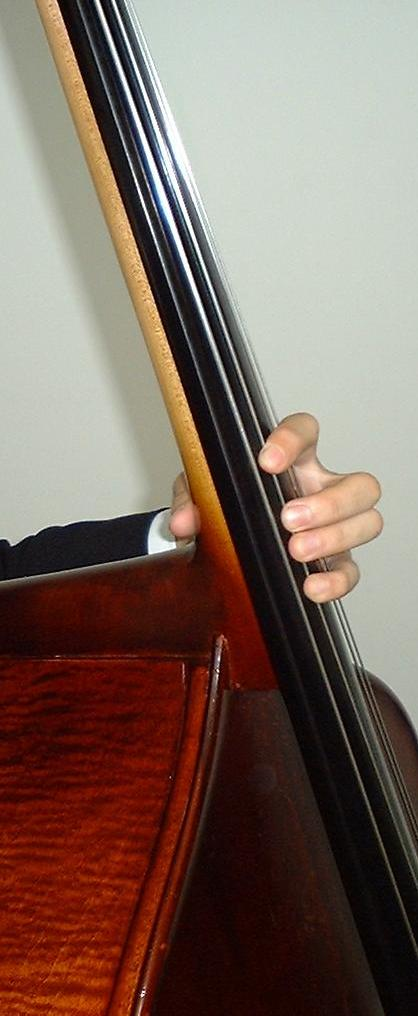
\includegraphics[height=6.5cm]{../Vol1/Pics/Position/4th_2.epsi}\\
{\flushleft\small 図\thefigure : 4th\(=\)ネックの一番下\\}
\end{center}
\end{minipage}
\hfill
\begin{minipage}{80pt}
\addtocounter{figure}{1}
\begin{center}
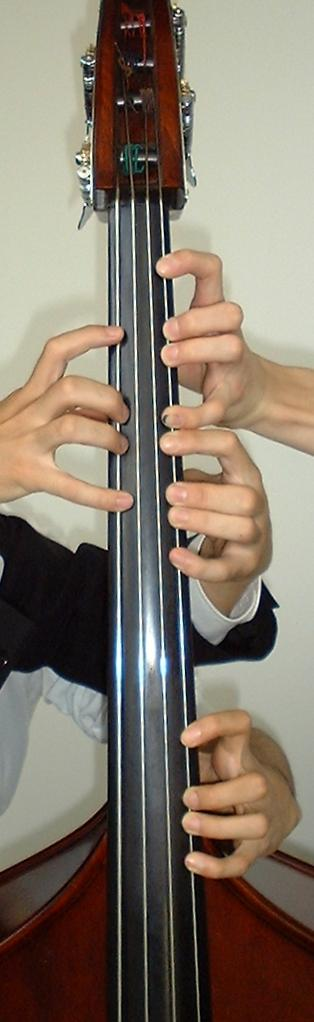
\includegraphics[height=6.5cm]{../Vol1/Pics/Position/4th_3.epsi}\\
{\flushleft\small 図\thefigure : 既出ポジションとの位置関係\\}
\end{center}
\end{minipage}
\end{flushleft}
\subsection{音階練習 \label{4th_scale}}
\begin{music}
\nostartrule
\parindent 0pt
\setclef1{\bass}  
\generalmeter{\meterC}
\generalsignature{-3}    
\startpiece
\notes\zchar{18}{変ホ長調(Es-dur)音階}\enotes
\NOtes\zchar{15}{half}\ovbkt{f}{3}{2}\zchar{7}{\bf 1}\ql{'E}\zchar{8}{\bf 4}\ql{F}\zchar{9}{\bf 0}\ql{G}\zchar{10}{\bf 1}\ql{!a}\enotes
\bar
\NOtes\zchar{17}{II}\ovbkt{'b}{1.1}{0}\zchar{11}{\bf 1}\ql{!b}\zchar{12}{\bf 4}\ql{c}\zchar{19}{IV}\ovbkt{'d}{3.4}{0}\zchar{13}{\bf 1}\ql{!d}\zchar{14}{\bf 2}\ql{e}\enotes
\bar
\NOtes\zchar{14}{\bf 2}\ql{e}\zchar{13}{\bf 1}\ql{d}\zchar{17}{II}\ovbkt{'b}{1.1}{0}\zchar{12}{\bf 4}\ql{!c}\zchar{11}{\bf 1}\ql{b}\enotes
\bar
\NOtes\zchar{16}{half}\ovbkt{'a}{3}{-3}\zchar{10}{\bf 1}\ql{!a}\zchar{9}{\bf 0}\ql{'G}\zchar{8}{\bf 4}\ql{F}\zchar{7}{\bf 1}\ql{E}\enotes
\setdoublebar\endpiece
\end{music}
\subsection{ハーフ、第I、第II、第IVポジションで弾ける名曲}
\subsubsection*{ワーグナー: 楽劇「ニュルンベルクのマイスタージンガー」 第1幕への前奏曲より}
\begin{music}
\nostartrule
\setclef1{\bass}
\generalsignature{0}    
\generalmeter{\meterfrac44}
\parindent 0pt
\startbarno=158
\def\writebarno{\tenrm\the\barno\barnoadd}
\def\raisebarno{2\internote}
\def\shiftbarno{0.1\Interligne}
\systemnumbers
\startpiece\bigaccid
\notes\zchar{18}{\LARGE \bf J}\zchar{20}{\hspace{2em} \bf aber sehr markiert}\zchar{16}{\hspace{2em}({\it ma molto marcato})}\enotes
\NOtes\zchar{-4}{I}\zchar{-8}{\mf}\zchar{12}{\downbow}\zchar{10}{\bf 2}\hu{'C}\zchar{10}{\upbow}\qup{!G}\zchar{8}{\upbow}\cu{!G}\enotes
\bar
\NOtes\islurd{0}{G}\zchar{8}{\downbow}\hu{G}\enotes
\notes\ibu{0}{G}{0}\tslur{0}{G}\qb{0}{GE}\zchar{-6}{half}\zchar{8}{\bf 1}\qb{0}{F}\tbu{0}\qb0{G}\enotes
\bar 
\Notes\qu{'AB}\zchar{-5}{II}\zchar{8}{\bf 1}\qu{C}\zchar{8}{\bf 4}\ql{D}\enotes
\bar
\Notes\zchar{-5}{I}\zchar{10}{\downbow}\zchar{8}{\bf 1}\ql{'E}\isluru{0}{F}\zchar{8}{\downbow}\ql{F}\enotes
\notes\ibl{0}{'F}{-3}\tslur{0}{F}\qb{0}{FE}\zchar{-6}{II}\zchar{8}{\bf 4}\qb{0}{D}\tbl{0}\zchar{8}{\bf 1}\qb{0}{C}\enotes
\bar
\NOtes\zchar{11}{\downbow}\zchar{8}{\bf 4}\hl{'D}\zchar{11}{\upbow}\zchar{8}{\bf 4}\qup{A}\zchar{11}{\upbow}\zchar{-5}{I}\zchar{8}{\bf 1}\cu{B}\enotes
\bar
\NOtes\islurd{0}{'C}\zchar{9}{\bf 2}\hu{C}\enotes
\notes\ibu{0}{'C}{1}\tslur{0}{C}\qb{0}{CB}\zchar{-5}{II}\zchar{11}{\bf 1}\qb{0}{C}\tbu{0}\qb{0}{D}\enotes
\bar
\notes\ibl{0}{'E}{0}\zchar{-6}{I}\zchar{8}{\bf 1}\qb{0}{EDE}\tbl{0}\zchar{-6}{II}\zchar{8}{\bf 1}\qb{0}{F}\enotes
\Notes\zchar{8}{\downbow}\ql{'G}\enotes
\notes\ibl{0}{'F}{-2}\zchar{-6}{I}\zchar{10}{\upbow}\zchar{8}{\bf 2}\qb{0}{F}\tbl{0}\zchar{8}{\upbow}\qb{0}{E}\enotes
\bar
\NOtes\isluru{0}{'D}\zchar{-6}{II}\zchar{8}{\bf 4}\hl{D}\enotes
\notes\ibl{0}{'D}{0}\tslur{0}{D}\qb{0}{DCD}\tbl{0}\zchar{-6}{I}\zchar{8}{\bf 1}\qb{0}{E}\enotes
\bar
\NOtes\zchar{14}{\bf allm\"{a}hlig immer st\"{a}rker}\zchar{-4}{({\it poco a poco pi\`u di forza})}\zchar{8}{\downbow}\hl{'F}\zchar{8}{\upbow}\qup{C}\zchar{8}{\upbow}\cu{C}\enotes
\bar
\notes\ibu{0}{'C}{0}\qb{0}{CAB}\tbu{0}\zchar{-4}{II}\zchar{11}{\bf 1}\qb{0}{C}\sk\enotes
\Notes\isluru{0}{'D}\hl{D}\enotes
\bar
\notes\ibu{0}{'D}{0}\tslur{0}{D}\qb{0}{D}\zchar{-4}{I}\zchar{12}{\bf 1}\qb{0}{BC}\tbu{0}\qb{0}{D}\sk\enotes
\Notes\isluru{0}{'E}\zchar{11}{\downbow}\zchar{8}{\bf 1}\hl{E}\enotes
\bar
\notes\ibl{0}{'E}{0}\tslur{0}{E}\qb{0}{E}\zchar{8}{\upbow}\qb{0}{CD}\tbl{0}\qb{0}{E}\ibl{0}{F}{0}\qb{0}{^FDE}\tbl{0}\qb{0}{F}\enotes
\bar
\Notes\ql{'G'A}\zchar{-4}{II}\zchar{12}{\bf 2}\ql{BC}\enotes
\bar
\Notes\zchar{-4}{IV}\unbkt{'A}{2.4}{0}\zchar{-8}{\it marcato}\zchar{15}{\downbow}\zchar{13}{\bf 1}\ql{!d}\isluru{0}{e}\zchar{16}{\downbow}\zchar{14}{\bf 4}\ql{e}\enotes
\notes\ibl{0}{e}{-4}\tslur{0}{e}\qb{0}{e}\zchar{13}{\bf 1}\qb{0}{d}\zchar{-4}{II}\zchar{12}{\bf 4}\qb{0}{c}\tbl{0}\qb{0}{b}\enotes
\bar
\Notes\zchar{-4}{I}\zchar{15}{\downbow\ \ \upbow}\zchar{13}{\bf 1}\uptext{\it tr}\wh{a}\enotes
\notes\multnoteskip\tinyvalue\tinynotesize\ibu{0}{'G}{4}\islurd{0}{G}\zchar{12}{\bf 0}\qb{0}{G}\tbu{0}\tslur{0}{!a}\zchar{13}{\bf 1}\qb{0}{!a}\enotes
\bar
\Notes\zchar{-4}{II}\zchar{12}{\downbow}\zchar{10}{\bf 4}\wh{'G}\enotes
\mulooseness=0
\setdoublebar\endpiece
\end{music}

